%! TEX program = xelatex
% Nécessaire pour la compilation pstricks
\documentclass[12pt]{article}                   % autres choix : report, book
\usepackage[a4paper]{geometry}                  % taille correcte du papier
\usepackage{silence}                            % Filtrer tous ces warnings ennuyeux
\usepackage[utf8]{inputenc}                     % encodage du fichier source
\usepackage[T1]{fontenc}                        % gestion des accents (pour les pdf)
\usepackage[french]{babel}                    % rajouter éventuellement english, greek, etc.
\usepackage{eurosym}                            % symbole euro

\usepackage{textcomp}                           % caractères additionnels
\usepackage{lmodern}                            % remplacer éventuellement par txfonts, fourier, etc.
\usepackage{amsmath,amssymb, amsthm}            % tout ce qu'il faut pour écrire des maths
\usepackage{dsfont}                             % Pour la fonction indactrice
\usepackage{xfrac}                              % fraction d'anneau

\usepackage{adforn}                             % Ornements header
\usepackage{yfonts}                             % Fontes gothiques supplémentaires
\usepackage{fourier-orns}                       % Ornements header
\usepackage{mathpazo}
\usepackage{pstricks,pst-plot,pstricks-add}     % tracer des fonctions
\usepackage[linesnumbered, french]{algorithm2e} % mise en page des algorithmes
\usepackage{tikz, tkz-euclide, tkz-tab}         % Dessiner aver tikz
\usetkzobj{all}                                 % et tout plein de paquets utiles
\usetikzlibrary{arrows.meta}
\usetikzlibrary{automata,positioning}
\usetikzlibrary{decorations.pathreplacing,calc}
\usetikzlibrary{arrows}
\usetikzlibrary{calc}
\usetikzlibrary{decorations.fractals}           % Dessiner les fractales usuelles
\usepackage{enumitem}                           % 1, 2, 3...
\usepackage{pgffor}                             % Pour faire des boucles

\usepackage{multicol}
\usepackage{comment}
\usepackage{subcaption}
\usepackage{array}                              % tableaux un peu plus paramétrables
%\usepackage{minted}
\usepackage[makestderr]{pythontex}
\usepackage[linesnumbered, french]{algorithm2e}

\usepackage{graphicx}                           % pour inclure des images
\usepackage{xspace}                             % protection des espaces
\usepackage{xcolor}                             % pour gérer les couleurs
\usepackage{microtype}                          % améliorations typographiques
\usepackage{hyperref}                           % gestion des hyperliens
\hypersetup{
    colorlinks = true,
    linkcolor = blue!50!gray!100!,
    linkbordercolor = {white},
}
\hypersetup{pdfstartview=XYZ}                   % Zoom hyperref
 
%%%%%%%%%%%
%% Maths %%
%%%%%%%%%%%
% Raccourcis pour les trucs longs à écrire. Reste d'Oxford principalement. 
\newcommand{\Prob}[2][]{\mathbb{P}_{#1}\left( #2 \right)}
\newcommand{\Exp}[2][]{\mathbb{E}_{#1}\left[ #2 \right]}
\newcommand{\Lawconv}{\stackrel{\mathcal{L}}{\longrightarrow}}
\newcommand{\Var}[1]{\mbox{Var}\left(#1 \right)}
\newcommand{\Card}[1]{\mbox{Card}\left(#1 \right)}
\newcommand{\Int}[4]{\int_{#1}^{#2} \! {#3} \, \mathrm{d}{#4}}
\newcommand{\kw}{\;|\;}
\newcommand{\im}{\textrm{Im}}
\newcommand{\disclamer}{\textit{L’usage de toute calculatrice, téléphone portable, ordinateur est strictement interdit. Un soin tout particulier devra être porté à la qualité et à la précision de la rédaction des argument } \vspace{1.cm}}
\newcommand{\legendeexos}{
\paragraph{Légende des exercices.}
\begin{center}
\begin{tabular}{cccc}
$\clubsuit$ : très flacile & $\varheart$ : à savoir par cœur & $\vardiamond$ : care aux calculs & $\spadesuit$ : qui s'y frotte s'y pique 
\end{tabular}
\end{center}
}

%%%%%%%%%%%%%%%%
%% Structures %%
%%%%%%%%%%%%%%%%

\newcounter{dfcount}
{\theoremstyle{definition} \newtheorem{definition}[dfcount]{Définition}}
\newcounter{propcount}
\newtheorem{propriete}[propcount]{Propriété}
\newcounter{thcount}
\newtheorem{theoreme}[thcount]{Théorème}
\newcounter{excount}
{\theoremstyle{definition} \newtheorem{exemple}[excount]{Exemple}}
\renewcommand{\theexemple}{\arabic{exemple}}
% Environnement exos
\newcounter{exoscount}
\newtheoremstyle{exercicestyle} % name of the style to be used
  {20pt}                        % measure of space to leave above the theorem. E.g.: 3pt
  {3pt}                         % measure of space to leave below the theorem. E.g.: 3pt
  {}                            % name of font to use in the body of the theorem
  {}                            % measure of space to indent
  {\bfseries}                   % name of head font
  {.}                           % punctuation between head and body
  {.5em}                        % space after theorem head; " " = normal interword space
  {}                            % Manually specify head
\theoremstyle{exercicestyle}
\newtheorem{exos}[exoscount]{Exercice}
\newenvironment{exo}[2]
  {
   \begin{exos}[#1]
   \leavevmode
   \marginpar{\hfill $#2 $ }}
  {\end{exos}}

\newenvironment{prob}{ \begin{center}
\Large{ \textsc{Problème}} \end{center} }{ \sepdown }

 % Théorèmes/propriétés avec un retour à la ligne.
\newtheoremstyle{break2}
  {\topsep}%   Space before theorem
  {\topsep}%   Space after theorem
  {\itshape}%  Body font
  {}%          Indent amount (empty = no indent, \parindent = para indent)
  {\bfseries}% Thm head font   
  {}%         Punctuation after thm head
  {.5em }%  Space after thm head (\newline = linebreak)
  {\thmname{#1}\thmnumber{ #2}\thmnote{ (#3)}.}% Thm head spec

\theoremstyle{break2}
\newtheorem{fbth}[thcount]{Théorème}
\newenvironment{bth}[1][]{\begin{fbth}[#1]\item\relax}{\end{fbth}}

\newtheorem{fbprop}[propcount]{Propriété}
\newenvironment{bprop}[1][]{\begin{fbprop}[#1]\item\relax}{\end{fbprop}}

 % Théorèmes/propriétés avec un retour à la ligne.
\newtheoremstyle{break3}
  {\topsep}%   Space before theorem
  {\topsep}%   Space after theorem
  {}%  Body font
  {}%          Indent amount (empty = no indent, \parindent = para indent)
  {\bfseries}% Thm head font   
  {}%         Punctuation after thm head
  {.5em }%  Space after thm head (\newline = linebreak)
  {\thmname{#1}\thmnumber{ #2}\thmnote{ (#3)}.}% Thm head spec

\theoremstyle{break3}
\newtheorem{fbdf}[dfcount]{Définition}
\newenvironment{bdef}[1][]{\begin{fbdf}[#1]\item\relax}{\end{fbdf}}

% Répéter un exercice n fois
\newcommand{\looped}[2]{
	\foreach \n in {1,...,#1}{
		#2
	}
}
%%%%%%%%%%%%%%%%%%
%% Mise en page %%
%%%%%%%%%%%%%%%%%%

\setlength{\textheight}{26.2cm}
\setlength{\textwidth}{17.0cm}
\setlength{\oddsidemargin}{-0.5cm}
\setlength{\evensidemargin}{0.0cm}
\setlength{\topmargin}{-2.0cm}
\pagestyle{empty}
\newif \ifnote
\notefalse
\reversemarginpar

\usepackage{titlesec}      % Interlignes pas trop gros
\titlespacing{\paragraph}{ %
  0pt}{                    % left margin
  1\baselineskip}{         % space before (vertical)
  1em}                     % space after (horizontal)

\usepackage{titlesec}
%\titleformat
%   {\section} % <command>
%   {\normalfont\Large\bfseries} % <format>
%   {\thesection} % <label>
%   {1em} % <sep>
%   {} % <before-code>
%\titleformat{\section}{\bfseries\sffamily\large}{\thesection.}{\hspace{1cm}}{}%
\titlespacing*                  % starred version: first paragraph is not indented
    {\section}                  % <command>
    {-22pt}                     % <left>
    {3.5ex plus 1ex minus .2ex} % <before-sep>
    {2.3ex plus .2ex}           % <after-sep>


\setlength{\columnseprule}{1pt}        % Séparateur vertical dans multicol
\def\columnseprulecolor{\color{black}} % De couleur noire.

% Type de colonnes pour array
\newcolumntype{P}[1]{>{\centering\arraybackslash}p{#1}}
\newcolumntype{M}[1]{>{\centering\arraybackslash}m{#1}}

% Filtrer les messages d'erreur kisoulent 
\WarningFilter{latex}{Marginpar on page}
\WarningFilter{latexfont}{Size}

%%%%%%%%%%%%%%%%%%%%%%%%%
%% Faire du joli latex %% 
%%%%%%%%%%%%%%%%%%%%%%%%%

% Faire des cœurs et des carreaux 
\DeclareSymbolFont{extraup}{U}{zavm}{m}{n}
\DeclareMathSymbol{\varheart}{\mathalpha}{extraup}{86}
\DeclareMathSymbol{\vardiamond}{\mathalpha}{extraup}{87}

% Police verbatim + souligné (links)
\usepackage[normalem]{ulem}
\useunder{\uline}{\ulined}{}%
\DeclareUrlCommand{\bulurl}{\def\UrlFont{\ttfamily\ulined}}

% Console Python. Les fichiers sont stockés dans ./pyfiles
\newcommand{\expandpyconc}[1]{\expandafter\reallyexpandpyconc\expandafter{#1}}
\newcommand{\reallyexpandpyconc}[1]{\pyconc{exec(compile(open('#1', 'rb').read(), '#1', 'exec'))}}

\newenvironment{pyconcodeblck}[1]%
 {\newcommand{\snippetfile}{./pyfiles/snippet-#1.py}
  \VerbatimEnvironment
  \begin{VerbatimOut}{\snippetfile}}%
 {\end{VerbatimOut}%
  \expandpyconc{\snippetfile}}


\begin{document}
%%%%%%%%%%%%%%%%%%%%%%
%% Header tout joli %%
%%%%%%%%%%%%%%%%%%%%%% 
\noindent\hrulefill
\raisebox{-2.1pt}[10pt][10pt]{\quad\decoone\quad}\hrulefill 

\leftline{$\textgoth{L}$ycée \hfill $\textgoth{I}$nformatique }
\hfill $\textgoth{S}$pécialité
 \begin{center}{\adforn{64}\quad \large{\textbf{ Algorithmique : algorithme des $k$ plus proches voisins }}\; \adforn{36}}\end{center}
\vspace{0.5cm}
\noindent
\hrulefill
\raisebox{-16.4pt}[10pt][10pt]{\begin{tikzpicture}[decoration=Koch snowflake]
\draw decorate{ decorate{ decorate{ decorate{ (6,-0) -- (4,0) -- (2,0) -- (0,0)  }}}};
\end{tikzpicture}}\hrulefill
\vspace{1cm}

\section*{Contexte}

Imaginons la situation suivante : il y a eu une fuite de produits chimiques dans un champ, et une partie du terrain a été contaminé et est devenu impropre à la culture. On a fait venir une équipe de scientifiques qui ont fait plusieurs prélèvements sur le terrain, et pour chacun des prélèvements ils ont indiqué si la zone était contaminée (zone rouge) ou saine (zone verte). Les scientifiques fournissent des données \textbf{annotées} (qu'on pourra appeler les données \textbf{d'apprentissage}, ou les données \textbf{connues}).

\begin{figure}[!h]
    \begin{subfigure}[b]{0.5\textwidth}
\begin{center}
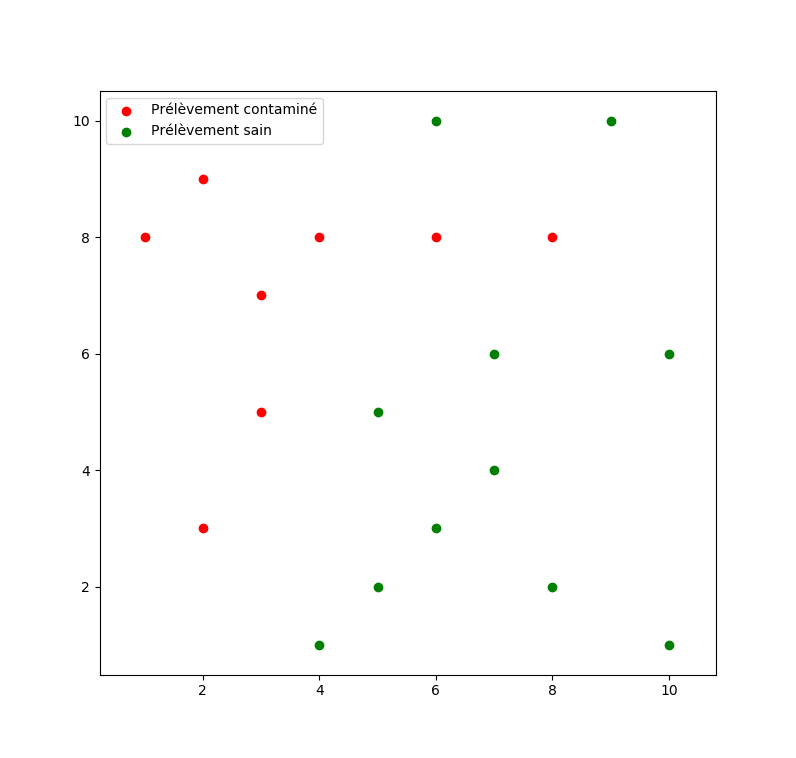
\includegraphics[width=9cm]{Figure_1.png}
\caption{Prélèvements des scientifiques}
\end{center}
    \end{subfigure}
    \begin{subfigure}[b]{0.5\textwidth}
\begin{center}
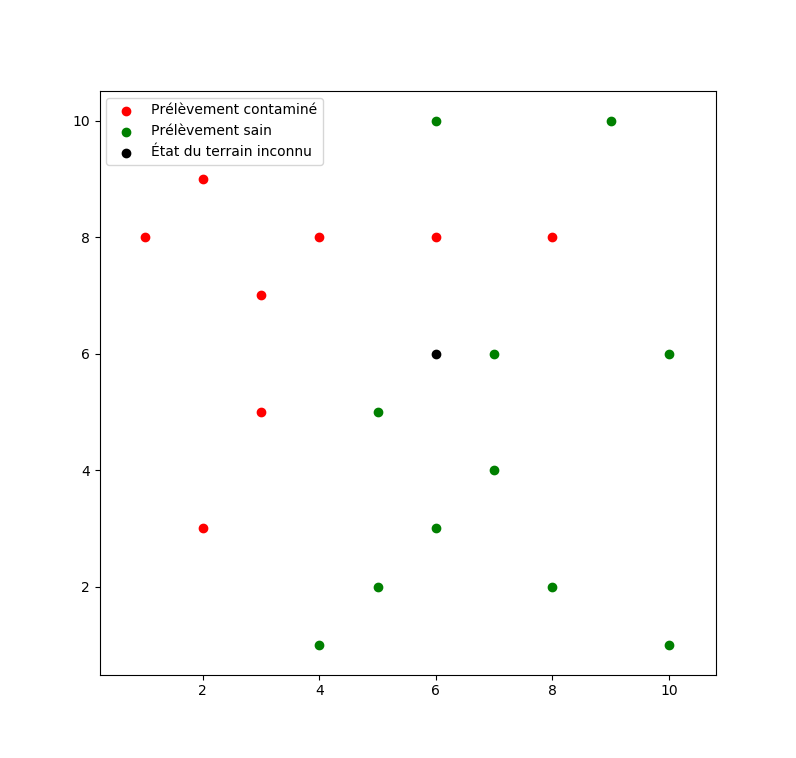
\includegraphics[width=9cm]{Figure_2.png}
\caption{Point à classer}
\label{fig:aclasser}
\end{center}
    \end{subfigure}
\end{figure}

La question est la suivante : l'agriculteur souhaite utiliser la parcelle de son terrain située aux coordonnées $(6, 6)$. Faire revenir les scientifiques est très couteux et n'est pas une solution acceptable, il doit donc trouver un moyen d'exploiter les données à sa disposition.



%\begin{figure}[!h]
%\begin{center}
%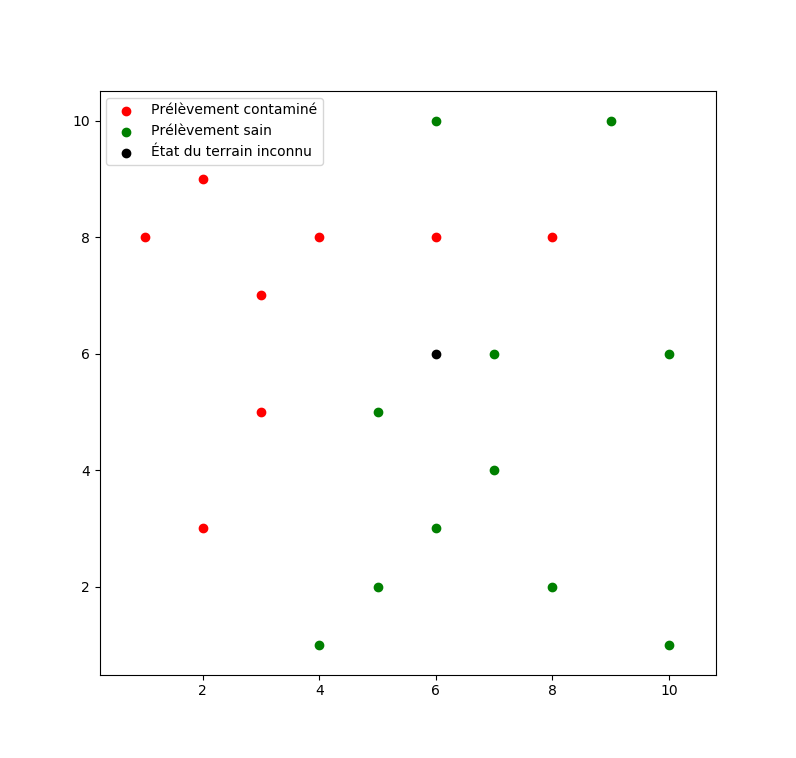
\includegraphics[width=10cm]{Figure_2.png}
%\label{fig:aclasser}
%\end{center}
%\end{figure}

\paragraph{Vocabulaire :} on appelle ce type de problème un problème de \textbf{classification} : il s'agit de classer dans une catégorie (contaminé/sain) une nouvelle donnée. La méthode se base sur un \textbf{apprentissage supervisé} : on connait déjà avec certitude la classe d'un certains nombre de données, et on veut déduire à partir de ces informations la classe de la nouvelle donnée. 

\section{Algorithme des $k$ plus proches voisins}

\begin{definition}
    
C'est un algorithme d'apprentissage supervisé qui peut permettre la classification de données. On appelle $X$ le point que l'on cherche à classer :
\begin{enumerate}
    \item calculer la distance entre $X$ et chacunes des données annotées ;
    \item trouver les $k$ données annotées dont la distance à $X$ est la plus faible (les $k$ plus proches voisins)
    \item renvoyer la classe majoritaire parmi les $k$ plus proches voisins.
\end{enumerate}
\end{definition} 

\begin{exemple}
    Reprennons l'exemple de la figure \ref{fig:aclasser}. On a utilisé l'algorithme des 3 plus proches voisins.  On rappelle la formule de la distance (euclidienne) entre deux points $A(x_A; y_A)$ et $B(x_B; y_B)$ du plan :
    $$ 
    d(A, B) = \sqrt{(x_B-x_A)^2 + (y_B - y_A)^2}.
    $$
Dans le cercle de centre $X(6, 6)$ se trouvent les 3 points les plus proches parmi les données d'apprentissage.    
    \begin{figure}[!h]
    \begin{center}
        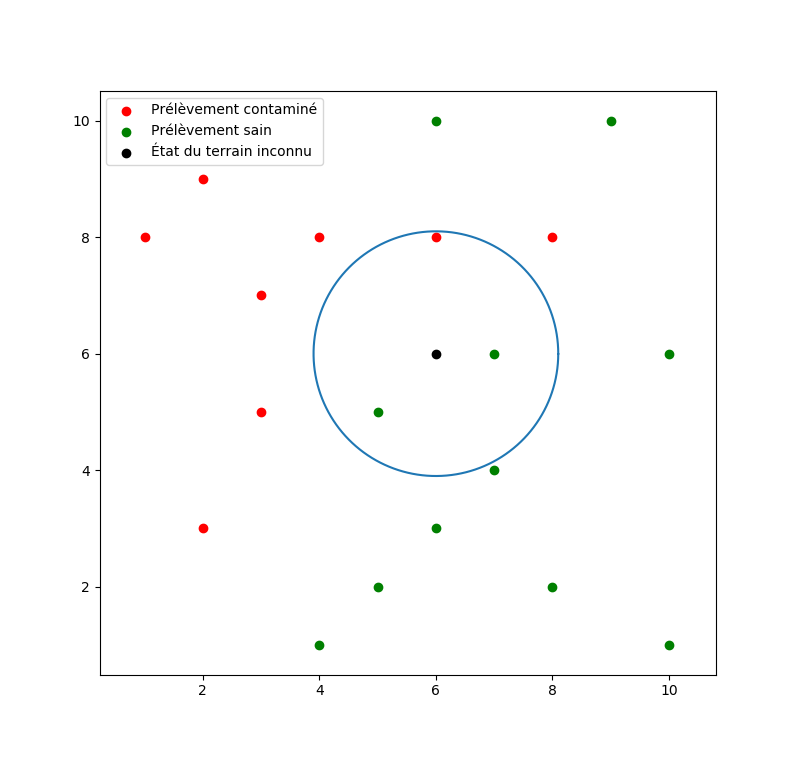
\includegraphics[width=10cm]{Figure_3.png}
        \caption{Voisinage du point dont on cherche la classe}
    \end{center}
    \end{figure}
    
    Parmi ces voisins, deux ont été étiquettés "sains" par les scientifiques, un seul a été étiquetté "contaminé". On peut selon toute vraisemblance penser qu'il s'agit d'une zone saine. 
\end{exemple}

\begin{exo}{}{  }
    Appliquer l'algorithme des plus proches voisins aux données suivantes. On évalue 12 élèves lors d'une épreuve sportive (le 100 mètre). On classe les élèves en deux groupes : les "sportifs" et les "non-sportifs". Ci-dessous les résultats de cette expérience.

    \begin{center}
        \renewcommand{\arraystretch}{1.5}
    \begin{tabular}{|M{2cm}|c|c|c|c|c|c|c|c|c|c|c|c|}
        \hline
        Temps (s) & $9,7$ & $9,85$ & $9,9$ & $10$ & $10,1$ & $10,1$ & $10,2$ & $10,2$ & $10,3$ & $10,5$ & $10,8$ & $11$ \\
    \hline
    Âge & 23 & 26 & 18 & 15 & 25 & 31 & 16 & 33 & 28 & 32 & 39 & 34 \\
    \hline 
    Classe & S & S & S & S & S & NS & S & NS & NS & NS & NS & NS \\
    \hline 
    \end{tabular}
    \end{center}

    \begin{enumerate}
        \item Représenter le nuage de points associé à ces données. $0,1$ sur l'axe des abscisses sera représenté par 1cm. $2$ sur l'axe des ordonnées sera représenté par 1cm. On prendra $9,5$ comme abscisse minimale, 11 comme abscisse maximale, 10 comme ordonnée minimale et 40 comme ordonnée maximale. On utilisera la couleur verte pour dénoter les sportifs et la couleur bleue pour dénoter les non-sportifs.
        \item Paul à 27 ans, et met 10 secondes à parcourir le 100m. Placer sur le graphique de la question précédente le point associé à Paul. 
        \item Si un candidat a $x$ ans et parcourt le 100m en $t$ secondes, la "distance" de ce candidat à Paul est donné par la formule :
            $$ 
            \sqrt{(27 - x)^2 + (10-t)^2}.
            $$
            Compléter le tableau suivant.
            \begin{center}
            \noindent \hspace{-1.2cm}\makebox[\textwidth]{
                \renewcommand{\arraystretch}{1.5}
    \begin{tabular}{|M{3cm}|c|c|c|c|c|c|c|c|c|c|c|c|}
        \hline
        Temps (s) & $9,7$ & $9,85$ & $9,9$ & $10$ & $10,1$ & $10,1$ & $10,2$ & $10,2$ & $10,3$ & $10,5$ & $10,8$ & $11$ \\
    \hline
    Âge & 23 & 26 & 18 & 15 & 25 & 31 & 16 & 33 & 28 & 32 & 39 & 34 \\
    \hline 
    Classe & S & S & S & S & S & NS & S & NS & NS & NS & NS & NS \\
    \hline 
    Distance à Paul & & & & & & & & & & & & \\
    \hline 
    \end{tabular}
}
            \end{center}
    \item Selon l'algorithme des $3$ plus proches voisins, Paul est-il plutôt sportif ou non ?

        \dotfill

        \dotfill
    \item Reprendre les questions précédentes avec Jacques, qui a 30 ans, et court lui aussi le 100m en 10 secondes. Quelle remarque pouvez-vous faire quant aux limites de l'algorithme ?
        

        \dotfill

        \dotfill

        \dotfill
    \end{enumerate}
    \label{exo:limites}

\end{exo} 

\paragraph{Une généralisation.} Comment faire dans le cadre de données plus complexes ? Imaginons une banque qui possède une liste de clients, répartis en 2 catégories : les clients "sûrs", et les clients "peu sûrs". Pour chacun des clients, 3 valeurs sont associées : l'âge, le salaire annuel en miliers d'euros, et le nombre de crédits. Les données possédées par la banque sont résumées dans le tableau suivant. 

\begin{center}
    \renewcommand{\arraystretch}{1.5}
   \begin{tabular}{|M{4cm}|c|c|c|c|c|c|}
       \hline
       Âge              & 50 & 40 & 30 & 45 & 18 & 60 \\
       \hline
       Salaire          & 48 & 36 & 96 & 30 & 24 & 24 \\
       \hline
       Nombre de crédit & 0 & 2 & 3 &1 & 2 &2 \\
       \hline
       Classe           &  S & PS & PS & S & PS & S \\
       \hline
   \end{tabular} 
\end{center}

Alexis, un nouveau client arrive à la banque. Il a 45 ans, gagne 33 000 euros par ans, et possède un crédit à charge. On aimerait savoir s'il peut être considéré comme sûr ou non. Si un client de la base de donnée de la banque a $x$ ans, gagne $s$ milliers d'euros et possède $n$ crédits, on peut définir la distance de ce client à Alexis par la formule :
$$
\sqrt{(45 - x)^2 + (33 - s)^2 + (1-n)^2}
$$
\begin{exo}{}{  }
    Appliquer l'algorithme des $3$ plus proches voisins pour déterminer si Alexis peut être considéré comme un client sûr ou non. 

    \noindent
        \dotfill

    \noindent
        \dotfill

    \noindent
        \dotfill

    \noindent
        \dotfill
\end{exo} 

\paragraph{Remarque.} Si les données possèdent $N$ caractéristiques (ou \textbf{composantes}), elles sont représentées par des "points" $A(a_1, \ldots, a_N)$ (une donnée), $B(b_1, \ldots, b_N)$ (une autre donnée), etc. La distance de $A$ à $B$ est alors donnée par la formule :
$$ 
d(A, B) = \sqrt{(b_1 - a_1)^2 + (b_2 - a_2)^2 + \ldots + (b_N - a_N)^2}.
$$

\section{Paramètres de l'algorithme}

\subsection{La valeur $k$}

$k$ est un paramètre de l'algorithme, définit par l'utilisateur. Différentes valeurs sont possibles.
\begin{itemize}[label=\textbullet]
    \item $k = 1$ : l'algorithme "colle" au maximum au données ;
    \item $k = 5$ : l'algorithme travaille "en moyenne" : il peut parfois être intéressant de se détacher des données pour avoir un point de vue plus "global" ;
    \item $k = +\infty $ : pas d'apprentissage, l'algorithme renvoie toujours la même classe car toutes les données sont considérées à chaque fois dans le vote.
\end{itemize}

\begin{figure}[!h]
    \begin{subfigure}[b]{5cm}
\begin{center}
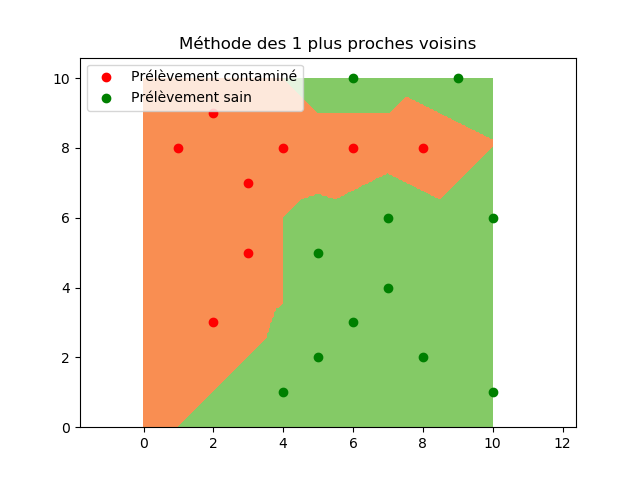
\includegraphics[width=6cm]{1NN.png}
\caption{$k = 1$}
\end{center}
    \end{subfigure}
    \begin{subfigure}[b]{5cm}
\begin{center}
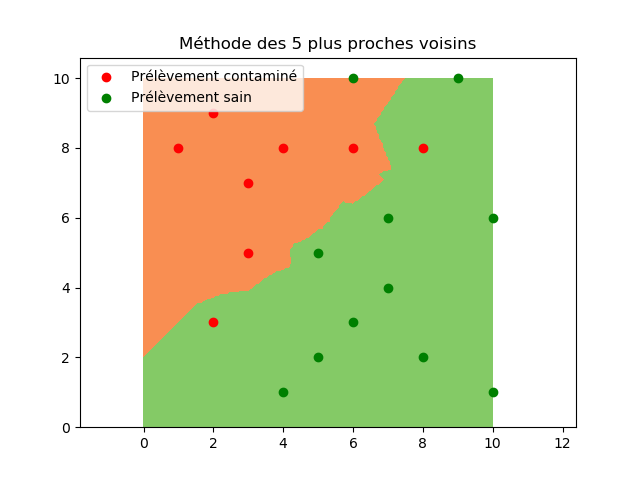
\includegraphics[width=6cm]{5NN.png}
\caption{$k = 5$}
\end{center}
    \end{subfigure}
    \begin{subfigure}[b]{5cm}
\begin{center}
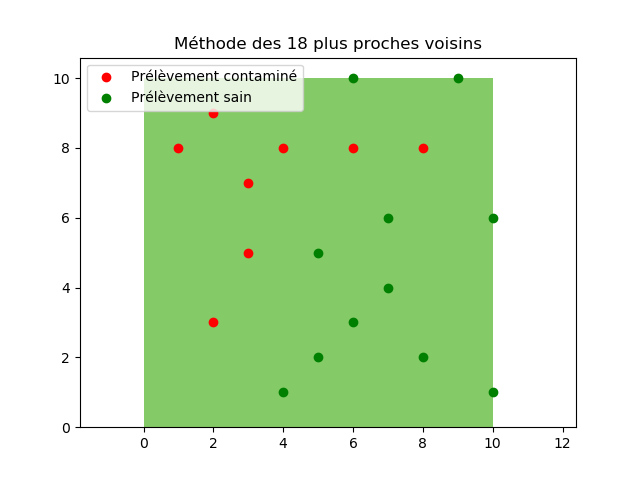
\includegraphics[width=6cm]{18NN.png}
\caption{$k = +\infty $}
\end{center}
    \end{subfigure}
    \caption{Influence de $k$}
\label{fig:kinfl}
\end{figure}


\subsection{Les données d'apprentissage}

Comme on l'a vu dans l'exercice \ref{exo:limites}, il est possible que l'algorithme prenne des décisions qui ne semblent pas raisonnables si les données ont été mal échantillonnées. L'échantillon d'apprentissage doit être le plus général possible, et doit représenter au maximum les différentes possibilités pour les données. 

\paragraph{Remarque.} Dans l'exercice \ref{exo:limites} toutes les personnes ayant moins de 26 ans étaient étiquettées "sportives" tandis que les personnes plus âgées étaient étiquettées "non sportives". Il y avait donc un biais dans notre algorithme ! Celui-ci apprennait en fait à distinguer si la personne était jeune ou non, ce qui n'était pas vraiment le but... 

Pour palier à cela nous aurions dû utiliser un jeu de données plus uniforme, en prennant en compte les personnes jeunes non sportives et les personnes moins jeunes sportives. 

\subsection{La distance}

Cet algorithme utilise la notion de "distance" pour trouver les voisins des éléments que l'on souhaite classer. Cette distance est là pour signifier à quel point les données "se ressemblent". Pour juger de la proximité de deux points $A(x_A, y_A)$ et $B(x_B, y_B)$, il n'est pas toujours judicieux d'utiliser la formule que l'on connait bien :
$$ 
d(A, B) = \sqrt{(x_B - x_A)^2 + (y_B-y_A)^2}.
$$
Le mathématicien décide parfois d'utiliser une autre "règle" pour mesurer les distances entre les objets. Avec son esprit tordu il appelle aussi cela "distance", même si ce n'est pas celle que vous connaissez. Par exemple on peut décider que :
$$ 
d(A, B) = |x_B - x_A| + |y_B - y_A|
$$
On appelle cette distance la distance de Manhattan, car c'est la distance que l'on parcourt à pied pour aller d'un point $A$ à un point $B$ dans les rues de Manhattan.

\begin{exos}
    Imaginons que nous avons représenté les rues de Manhattan par le quadrillage suivant. Chaque arrête du quadrillage symbolise une rue, les piétons ne peuvent se déplacer \textbf{que} sur les arêtes. L'unité est la dizaine de mètres.

\begin{center}\centering
	\psset{algebraic=true,%
		xunit=0.8cm, 
		yunit=0.8cm, 
		linewidth=0.3pt,
		yMaxValue=6.5,
		yMinValue=-4.5,
	plotpoints=1000}
	\begin{pspicture}*(-1.5, -1.5)(8.5, 6.5)
		\psgrid[gridwidth = 0pt, gridcolor=gray, subgriddiv = 0, gridlabels=0pt, xunit = 1, yunit = 1](-1.5,-1.5)(9.5, 7.5)
		\psaxes[Dx=1,Dy=1,xticksize=3pt ,yticksize=-3pt, arrowsize = 4pt ]{->}(0,0)(-3.5,-4.5)(8.5,6.5)
		\uput[90](8, 0){$x$}
		\uput[0](0, 6){$y$}
		\psdot[dotstyle=+, dotsize=5pt](2, 1)
		\uput[45](2, 1){$A$}
		\psdot[dotstyle=+, dotsize=5pt](7, 5)
		\uput[45](7, 5){$B$}
	\end{pspicture}
\end{center}
\begin{enumerate}
    \item Un piéton part du point $A$ et se rend au point $B$, quelle distance parcourt-il ? Après avoir indiqué les coordonnées respectives de $A$ et de $B$, comparer avec la formule :
$$ 
d(A, B) = |x_B - x_A| + |y_B - y_A|
$$

\dotfill

\dotfill

\dotfill

    \item Un oiseau part du point $A$ et se rend au point $B$, quelle distance parcourt-il ? Quelle formule avez-vous utilisé ?

\dotfill

\dotfill

\dotfill
\end{enumerate}
    
\end{exos}

\end{document}
 
